%%%%%%%%%%%%%%%%%%%%%%%%%%%%%%%%%%%%%%%%%%%%%%%%%%%%%%
% A Beamer template for University of Wollongong     %
% Based on THU beamer theme                          %
% Author: Qiuyu Lu                                   %
% Date: July 2024                                    %
% LPPL Licensed.                                     %
%%%%%%%%%%%%%%%%%%%%%%%%%%%%%%%%%%%%%%%%%%%%%%%%%%%%%%

\documentclass[serif,8pt, aspectratio=169]{beamer}
%\documentclass[serif]{beamer}  % for 4:3 ratio
\usepackage[T1]{fontenc} 
\usepackage{fourier} % see "http://faq.ktug.org/wiki/uploads/MathFonts.pdf" for other options
\usepackage{hyperref}
\usepackage{latexsym,amsmath,xcolor,multicol,booktabs,calligra}
\usepackage{graphicx,pstricks,listings,stackengine,animate}
\usepackage{lipsum}
\usepackage{multirow}

\author{Thiago E. Fernandes, Marcelo Lobosco, Rodrigo W. dos Santos}
\title{First Insights into PINNs for Accelerating Immune Response Models}
\institute{
    Postgraduate in Computational Modeling \\
    Federal University of Juiz de Fora
}
\date{\small \today}
\usepackage{UoWstyle}

% defs
\def\cmd#1{\texttt{\color{red}\footnotesize $\backslash$#1}}
\def\env#1{\texttt{\color{blue}\footnotesize #1}}
\definecolor{deepblue}{rgb}{0,0,0.5}
\definecolor{deepred}{RGB}{153,0,0}
\definecolor{deepgreen}{rgb}{0,0.5,0}
\definecolor{halfgray}{gray}{0.55}

\lstset{
    basicstyle=\ttfamily\small,
    keywordstyle=\bfseries\color{deepblue},
    emphstyle=\ttfamily\color{deepred},    % Custom highlighting style
    stringstyle=\color{deepgreen},
    numbers=left,
    numberstyle=\small\color{halfgray},
    rulesepcolor=\color{red!20!green!20!blue!20},
    frame=shadowbox,
}


\begin{document}

\begin{frame}
    \titlepage
    \vspace*{-0.6cm}
    \begin{figure}[htpb]
        \begin{center}
            
\includegraphics[keepaspectratio, scale=0.13]{pic/UFJF.png}
        \end{center}
    \end{figure}
\end{frame}

\begin{frame}    
\tableofcontents[sectionstyle=show,
subsectionstyle=show/shaded/hide,
subsubsectionstyle=show/shaded/hide]
\end{frame}

\section{Problem Formulation}

\subsection{Mathematical model}
    \begin{frame}[fragile]{Mathematical model}
        \begin{minipage}{0.55\linewidth}
            \centering % \includegraphics{}
             \animategraphics[width = 0.9\linewidth, autoplay, loop]{2}%frame rate
            {anims/Chemotaxis}%path to figures
            {1}%start index
            {57}%end index
        \end{minipage}
        \begin{minipage}{0.4\linewidth}
            The mathematical model used to describe the pathophysiology of edema formation was proposed in a previous work \cite{reis2019mathematical,reis2019personalized}. This model includes the inflammatory part which describes the interaction between a pathogen and the human immune system.
            
            The pathogen is modelled by:
            \begin{equation}
            \left\{\begin{matrix}
             \frac{d(\phi_fC_b)}{dt}=-r_b+q_b,~t\in(0,10]\\
             C_b(0) = \delta_b,
            \end{matrix}\right.
            \end{equation}

            where 
            
            \begin{equation}
                q_b = c_b C_b
            \end{equation}

            \begin{equation}
                r_b = \lambda_{nb}C_nC_b
            \end{equation}
        \end{minipage}
    \end{frame}

    \begin{frame}[fragile]{Mathematical model}
        \begin{minipage}{0.55\linewidth}
            \centering % \includegraphics{}
             \animategraphics[width = 0.9\linewidth, autoplay, loop]{2}%frame rate
            {anims/Chemotaxis}%path to figures
            {1}%start index
            {57}%end index
        \end{minipage}
        \begin{minipage}{0.4\linewidth}
            The leukocyte differential model is represented by:

            \begin{equation}
            \left\{\begin{matrix}
             \frac{d(\phi_fC_n)}{dt}=-r_n+q_n,~t\in(0,10]\\
             C_b(0) = 0
            \end{matrix}\right.
            \end{equation}

            where 
            
            \begin{equation}
                q_n = \gamma_nC_b(C_{n,max}-C_n)
            \end{equation}

            \begin{equation}
                r_b = \lambda_{bn}C_nC_b+\mu_nC_n
            \end{equation}
        \end{minipage}
    \end{frame}

    \begin{frame}[fragile]{Mathematical model}
        \begin{figure}
            \centering
            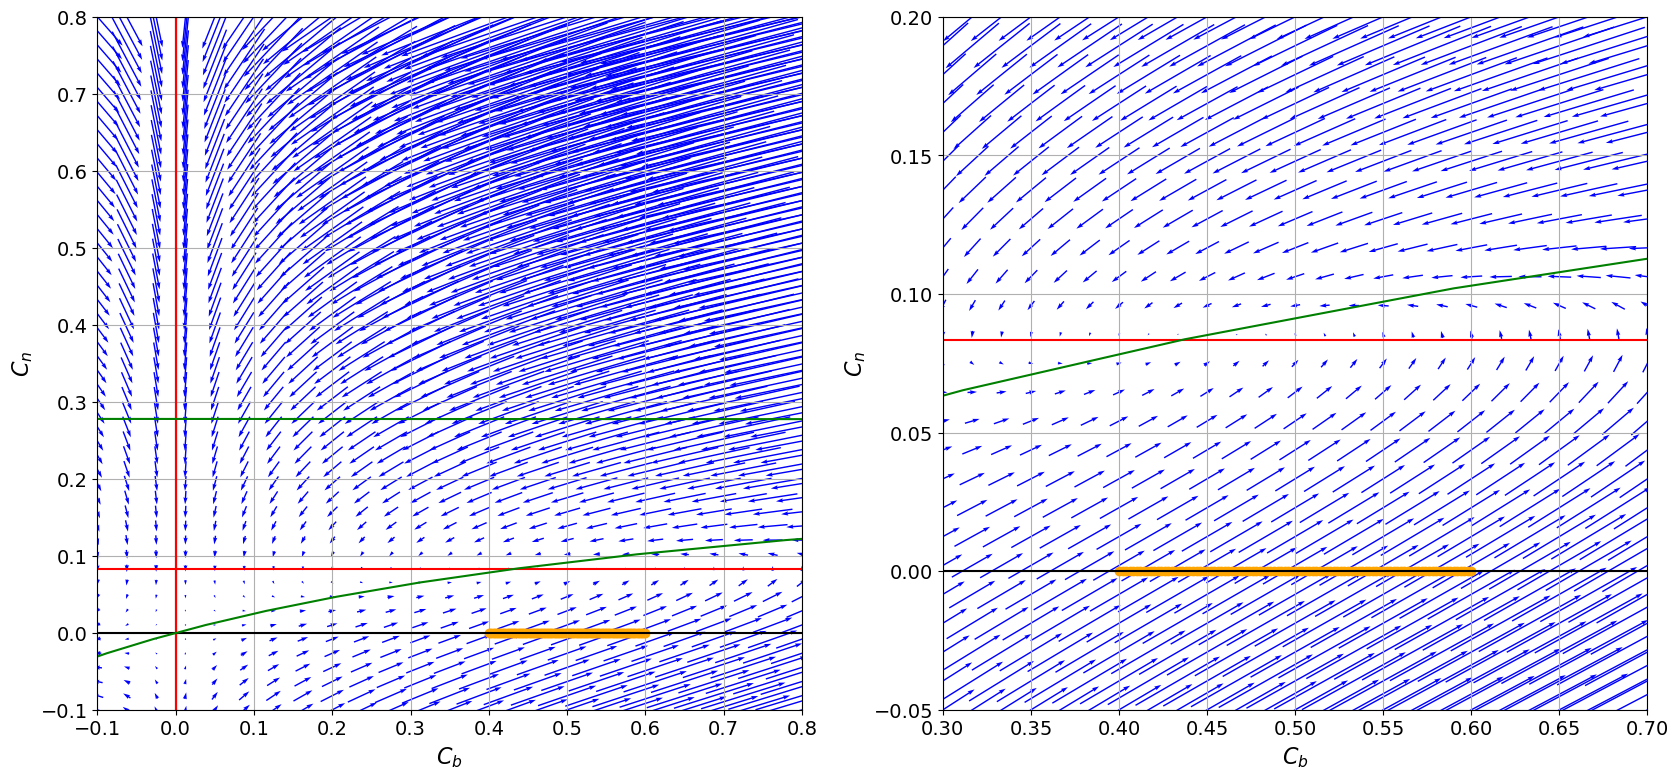
\includegraphics[width=0.8\linewidth]{pic/phase_plane.png}
            \caption{Phase plane for the system of equations.}
            \label{fig:phase-plane}
        \end{figure}
    \end{frame}

\subsection{Physics-Informed Neural Networks (PINN)}
 
\begin{frame}[fragile]{Physics-Informed Neural Networks (PINN)}
    \begin{figure}
        \centering
        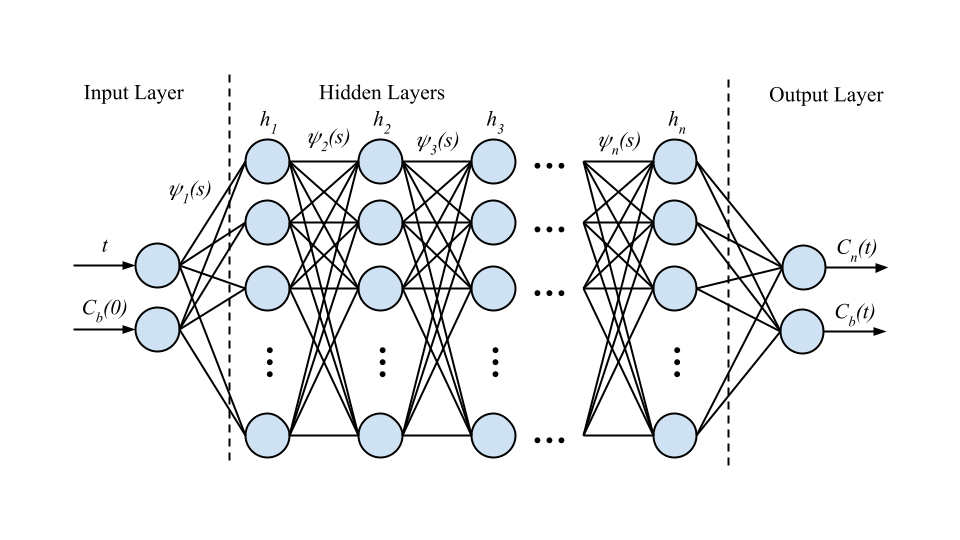
\includegraphics[width=0.8\linewidth]{pic/Imune_pinn_model.png}
        \caption{Neural Networks architecture.}
        \label{fig:pinn-selection}
    \end{figure}
\end{frame}

\begin{frame}[fragile]{Physics-Informed Neural Networks (PINN)}
    In alignment with the foriginal formulation of Raissi et al. \cite{raissi2019physics}, we generaly consider PDEs taking the form
    
    \begin{equation}
        \frac{\partial u}{\partial t} + \Phi[u] = 0,~t\in [0,T],~x \in \Omega
    \end{equation}
    
    subject to the initial and boundary conditions
    
    \begin{equation}
        u(0,x)=g(x),~x\in\Omega 
    \end{equation}
    
    \begin{equation}
        \beta [u]=0,~t\in[0,T],~x\in\partial\Omega
    \end{equation}

    This formulation enables us to define the PDE residuals as follows:

    \begin{equation}
        \zeta_\theta (t,x) = \frac{\partial u_\theta}{\partial t}(t,x) + \Phi[u_\theta](t,x)
    \end{equation}

    
\end{frame}

\begin{frame}[fragile]{PINN architecture grid-search}
    Consequently, a physics-informed model is trained by minimising the following composite loss function:
    
    \begin{equation}
       \textit{L}(\theta ) = \textit{L}_{ic}(\theta )+\textit{L}_{bc}(\theta )+\textit{L}_{r}(\theta )+\textit{L}_{dt}(\theta )
    \end{equation}
    
    \begin{equation}
        \textit{L}_{ic}(\theta )=\frac{1}{N_{ic}}\sum^{N_{ic}}_{i=1}\sqrt{(u_\theta(0,x_{ic}^i)-g(x_{ic}^i))^2}
    \end{equation}

    \begin{equation}
        \textit{L}_{bc}(\theta )=\frac{1}{N_{bc}}\sum^{N_{bc}}_{i=1}\sqrt{\beta[u_\theta](t^{i}_{bc},x^i_{bc})^2}
    \end{equation}

    \begin{equation}
        \textit{L}_{r}(\theta )=\frac{1}{N_{r}}\sum^{N_{r}}_{i=1}\sqrt{(\zeta_\theta(t^i_{r},x^i_{bc})^2}
    \end{equation}

    \begin{equation}
        \textit{L}_{dt}(\theta )=\frac{1}{N_{dt}}\sum^{N_{dt}}_{i=1}\sqrt{(u_\theta(t^i_{dt},x_{dt}^i)-u(t^i_{dt},x_{dt}^i))^2}
    \end{equation}

\end{frame}

%where $\Phi[u]$ represents a linear or nonlinear differential operator, and B[⋅] denotes a boundary operator associated with Dirichlet, Neumann, Robin, or periodic boundary conditions. Furthermore, u represents the unknown latent solution governed by the PDE system described by Equation (2.1). We proceed by approximating the unknown solution u(t,x) with a deep neural network (t,x), where θ encompasses all adjustable parameters of the network, such as weights and biases. 

\section{Results}
    \subsection{PINN architecture grid-search}
    \begin{frame}[fragile]{PINN architecture grid-search}
        \begin{minipage}{0.55\linewidth}
            \begin{figure}
                \centering
                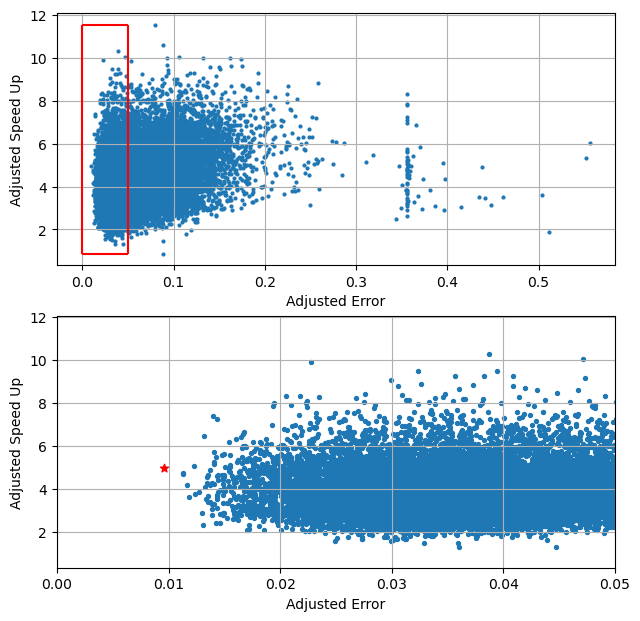
\includegraphics[width=0.85\linewidth]{pic/pinn_selection.png}
                \caption{Adjusted error and speed up of the tested architectures.}
                \label{fig:pinn-selection}
            \end{figure}
        \end{minipage}
        \begin{minipage}{0.4\linewidth}
            The adjusted error and speedup are defined respectively by Equations \ref{eq:aj-error} and \ref{eq:aj-speed}.
    
            \begin{equation}\label{eq:aj-error}
                E_{aj} = RMSE + RSE_{max}
            \end{equation}
    
            \begin{equation}\label{eq:aj-speed}
                S_{aj} = \left< S \right>_{av} - \sigma_s
            \end{equation}
    
            where $RMSE$ stands for Root Mean Squared Error and $S$ is the speed up.
        \end{minipage}
    \end{frame}
    
    \begin{frame}[fragile]{PINN architecture grid-search}
        \begin{minipage}{0.55\linewidth}
            \begin{figure}
                \centering
                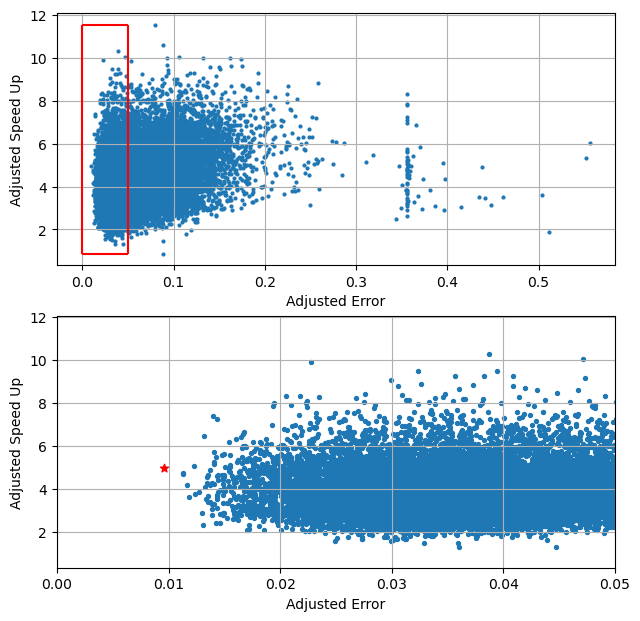
\includegraphics[width=0.85\linewidth]{pic/pinn_selection.png}
                \caption{Adjusted error and speed up of the tested architectures.}
                \label{fig:pinn-selection}
            \end{figure}
        \end{minipage}
        \begin{minipage}{0.44\linewidth}
            Considering the 22465 architectures studied, the chosen one is composed by 4 hidden layers with 16, 8, 32, and 16 neurons respectively. Considering the PyTorch documentation, \cite{pytorch}, the activation functions are defined as:
    
            
            \begin{equation}
                \psi_1= \frac{sinh(x)}{cosh(x)} 
            \end{equation}
    
            \begin{equation}
                \psi_2= x\cdot \sigma(x)
            \end{equation}
    
            \begin{equation}
                \psi_3= \psi_4 = max(0,x)
            \end{equation}
    
            where $x$ represents the values from the previous layers and  $\sigma(x)$ is the logistic sigmoid function.
        \end{minipage}
    \end{frame}
\subsection{PINN and NN comparison}

\begin{frame}[fragile]{PINN and NN comparison}

    \begin{figure}
        \centering
        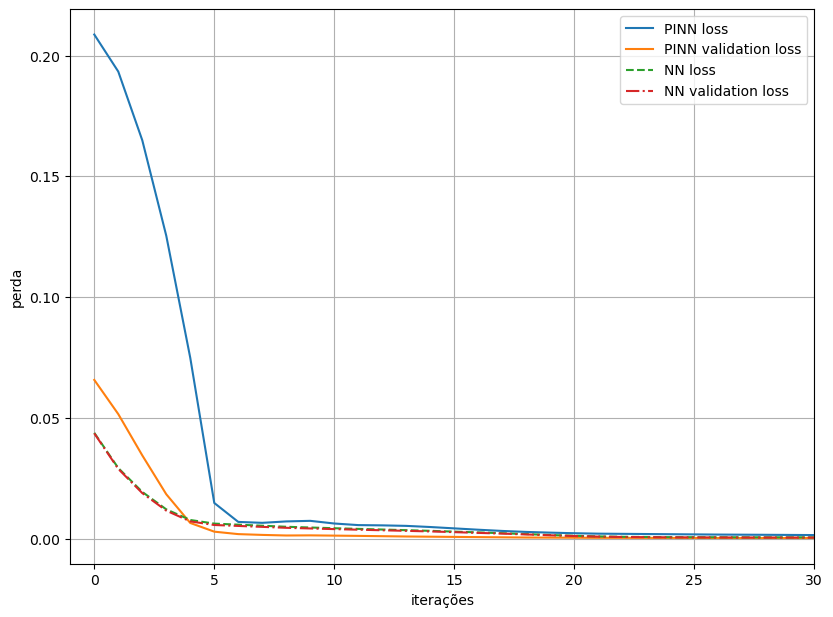
\includegraphics[width=0.95\linewidth]{pic/learning_curves.png}
        \caption{Learning curves for the NN and PINN training.}
        \label{fig:enter-label}
    \end{figure}

\end{frame}

\begin{frame}[fragile]{PINN and NN comparison}

    \begin{figure}
        \centering
        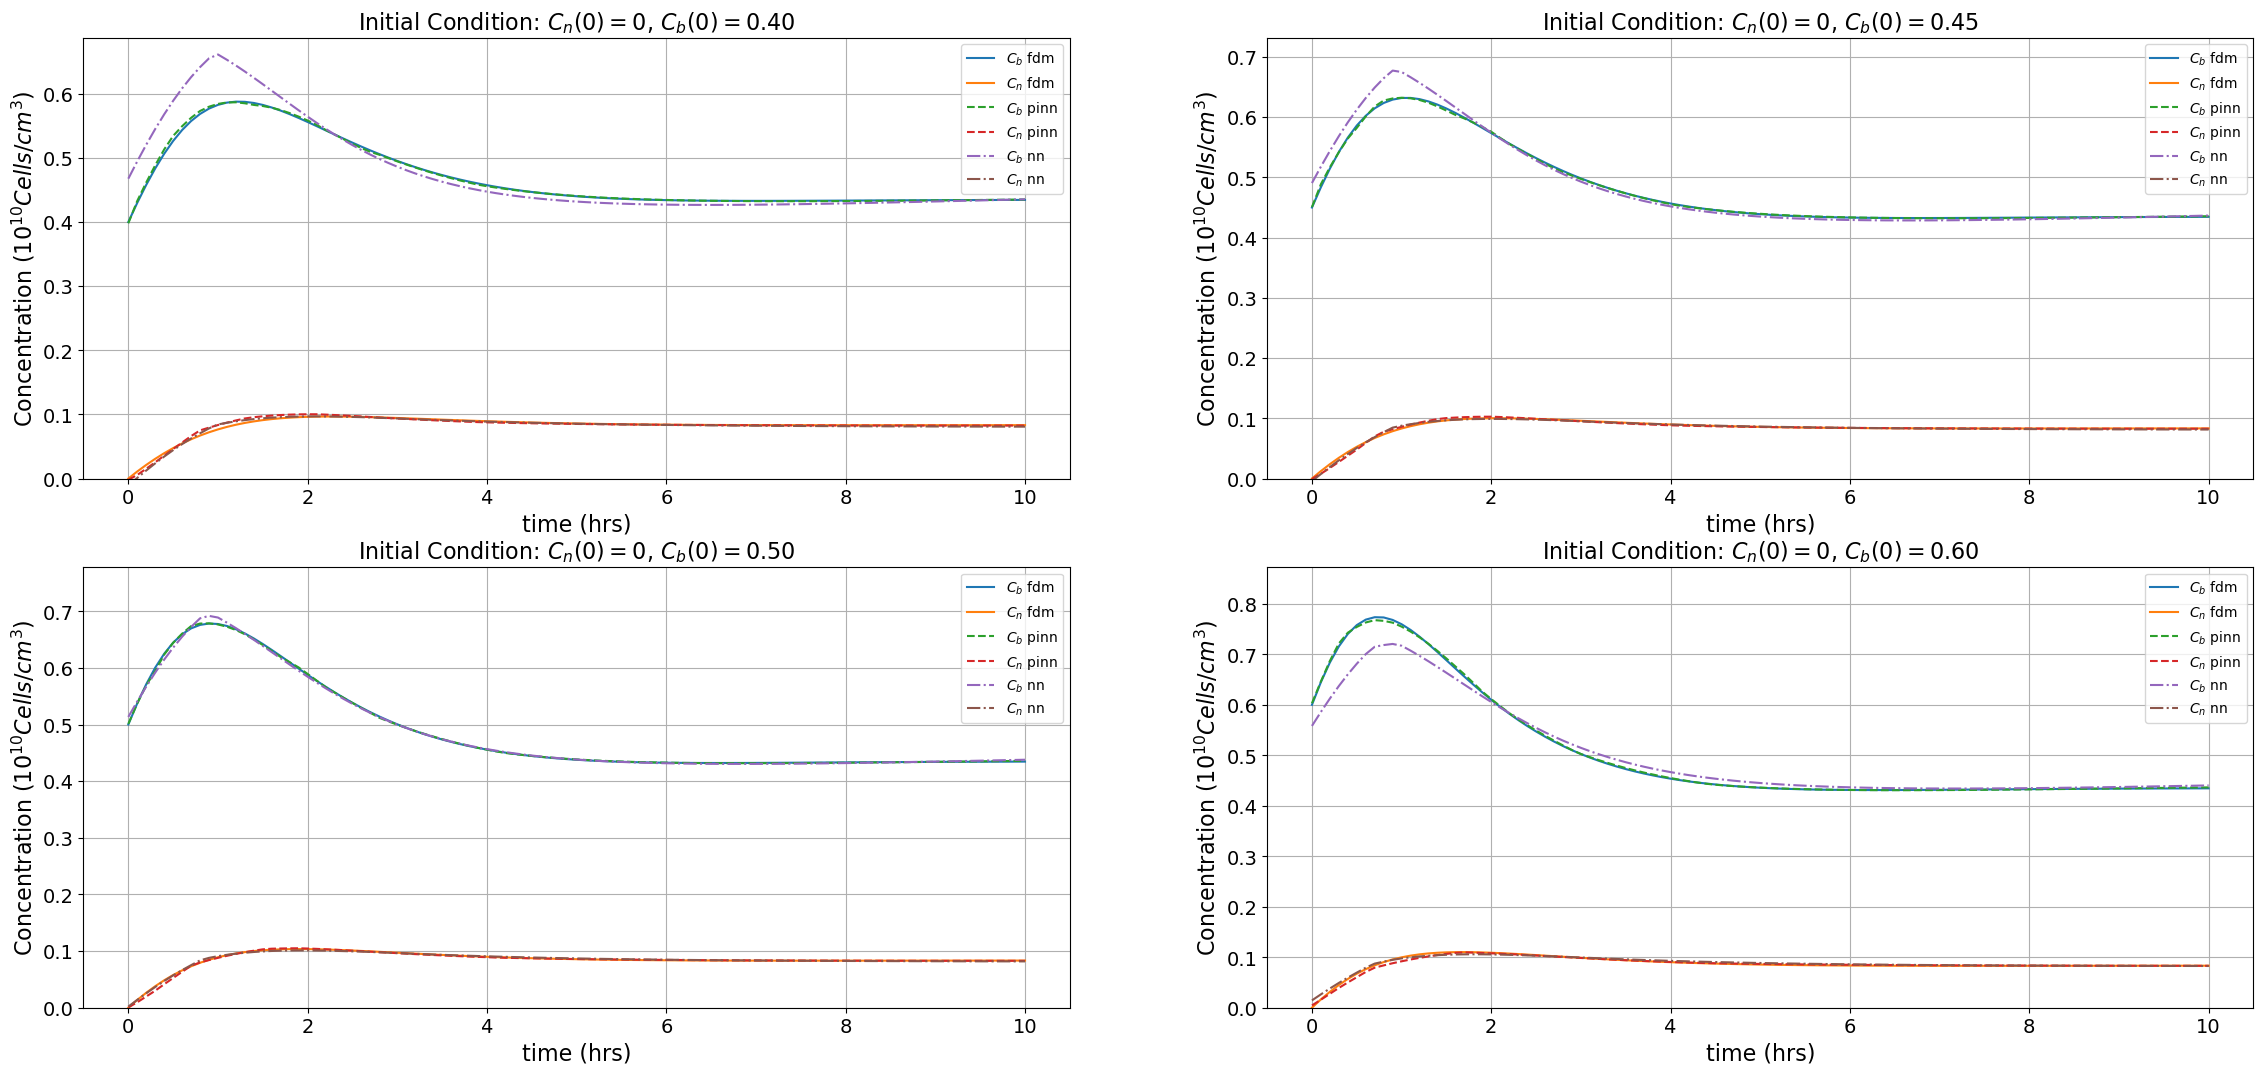
\includegraphics[width=0.95\linewidth]{pic/conc_curve_plot.png}
        \caption{Concentration curves for the different computational models}
        \label{fig:enter-label}
    \end{figure}

\end{frame}

\begin{frame}[fragile]{PINN and NN comparison}
    \begin{figure}
        \centering
        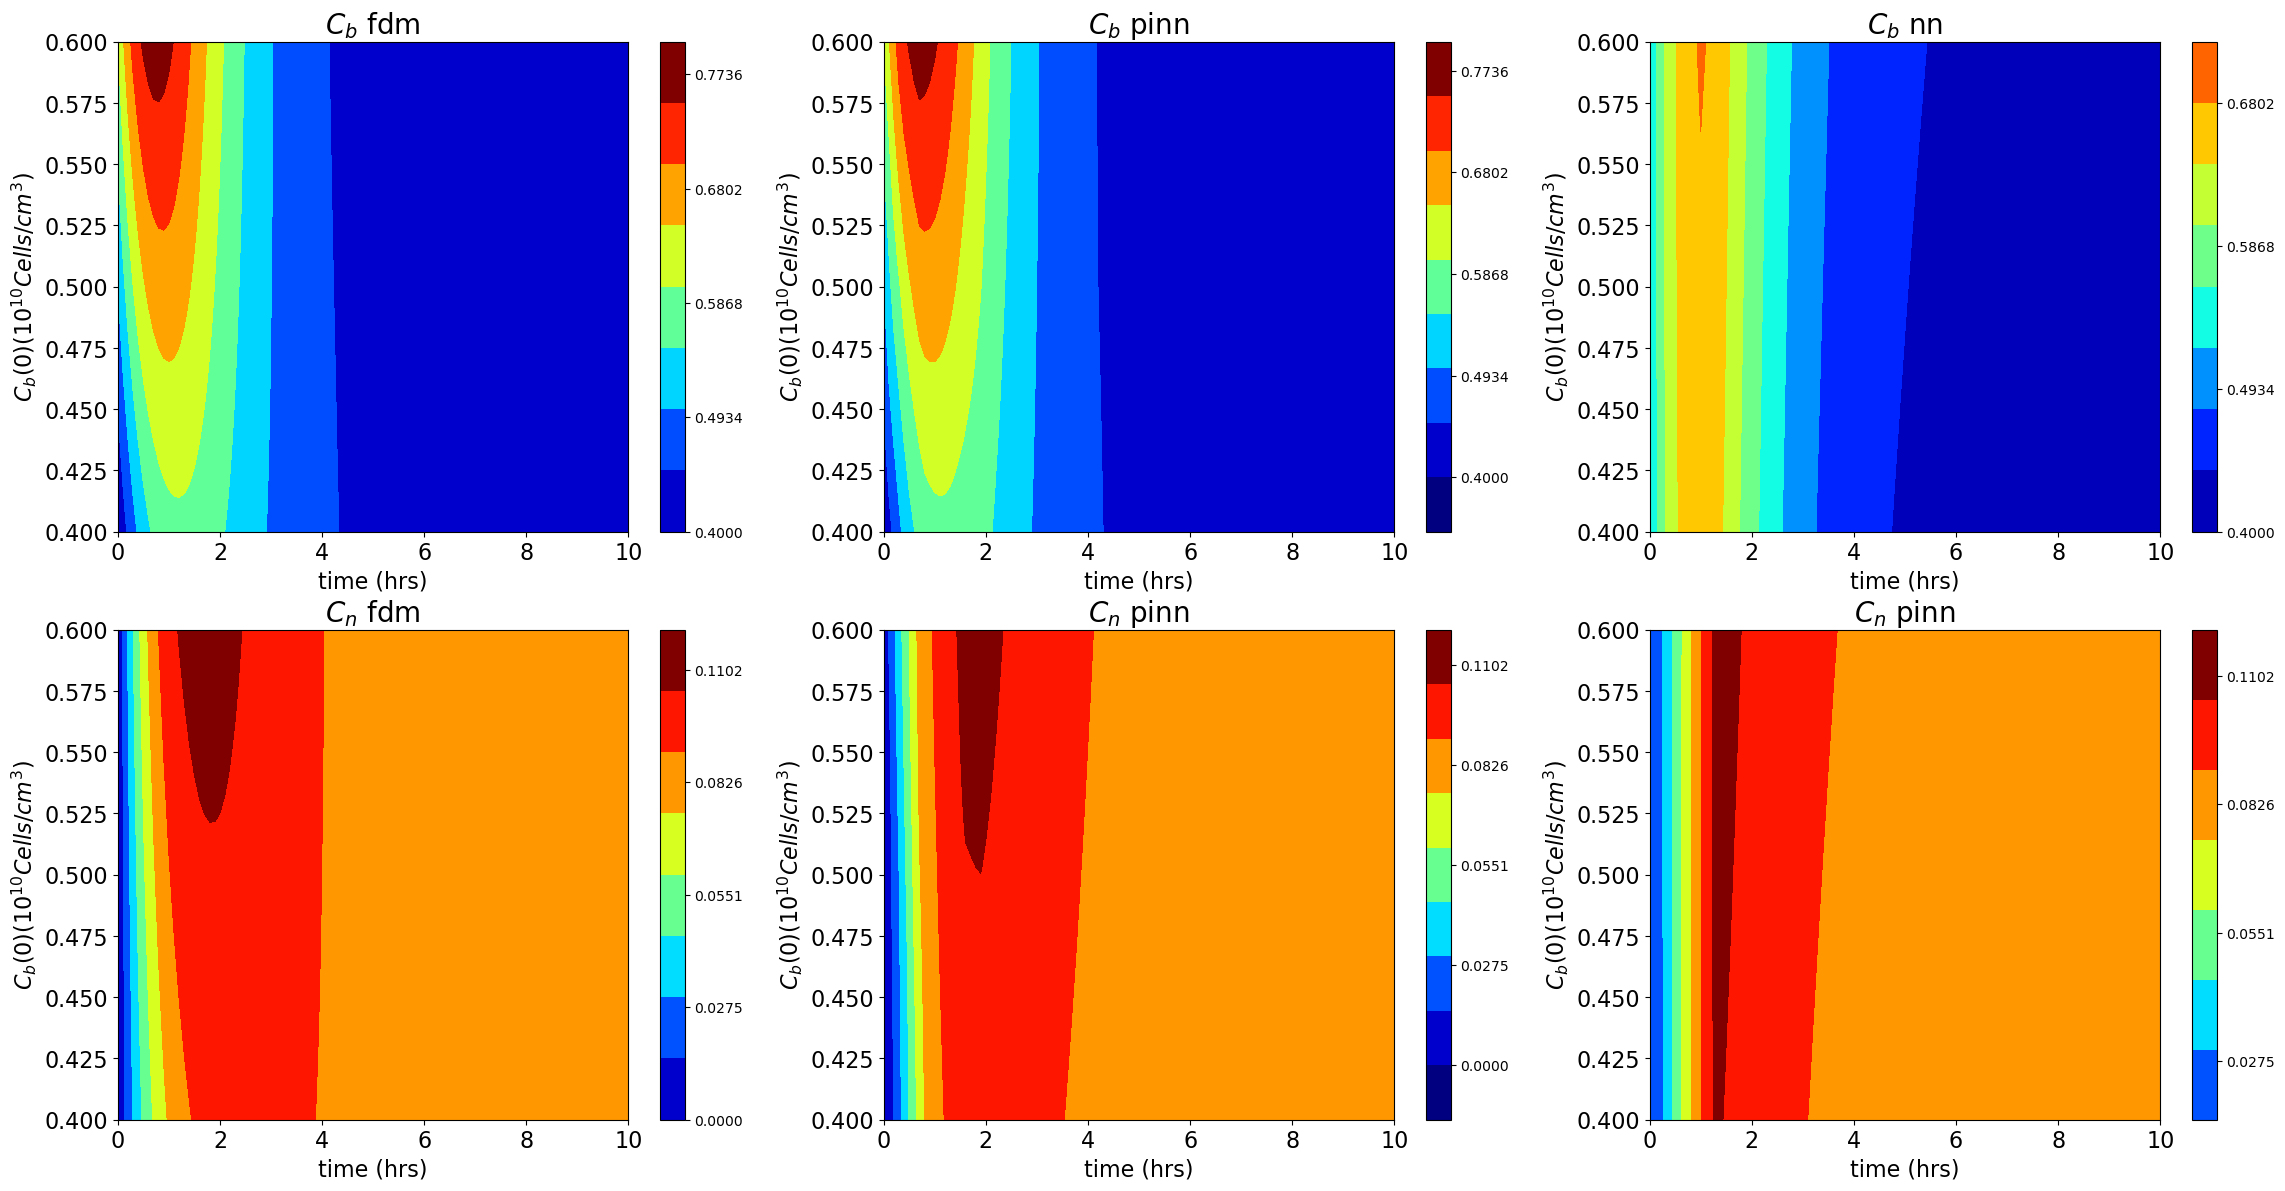
\includegraphics[width=0.95\linewidth]{pic/conc_heat_plot.png}
        \caption{Concentration heat-map for the different computational models}
        \label{fig:enter-label}
    \end{figure}
\end{frame}

\begin{frame}[fragile]{PINN and NN comparison}

    Table \ref{tab:results} presents the results for the PINN and NN.
    
        \begin{table}[htb!]
        \centering
        \caption{Experimental results of PINN constrains implementation}
        \label{tab:results}
        \begin{tabular}{ccccc}
        \cline{1-5}
        Model & RMSE        & $RSE_{max}$ & Mean speed up              & Speed up Standard Deviation \\ \cline{1-5}
        PINN  & 0.001530657 & 0.0080879815   & \multirow{2}{*}{5.9304240} & \multirow{2}{*}{0.96761669} \\
        NN    & 0.11618373   & 0.14936338     &                            &                            
        \end{tabular}
        \end{table}

\end{frame}

\section{References}

\begin{frame}[allowframebreaks]
    \bibliography{ref}
    \bibliographystyle{IEEEtran}
    %\nocite{*} % used here because no citation happens in slides
    % if there are too many try use:
    % \tiny\bibliographystyle{alpha}
\end{frame}


\begin{frame}
    \begin{center}
        {\Huge\calligra Thank You}
    \end{center}
\end{frame}

\end{document}